\documentclass[12pt]{article}

\usepackage[spanish]{babel}
\usepackage{hyperref}
\usepackage{graphicx}
\usepackage{listings}
\usepackage{color}
\usepackage{multicol}
\usepackage{amssymb}
\spanishdecimal{.}
%% Título
\title{Matemáticas para las Ciencias Aplicadas I}

%% Fecha
\date{\today}

%% Autor
\author{Flores Morán Julieta Melina \\ Zarco Romero José Antonio}


%% Se marca el inicio del documento.
\begin{document}

%% Comando para crear el título.
\maketitle

\section{La edad de la sábana santa}
Zarco Romero José Antonio\\

\begin{figure}[h]
\centering
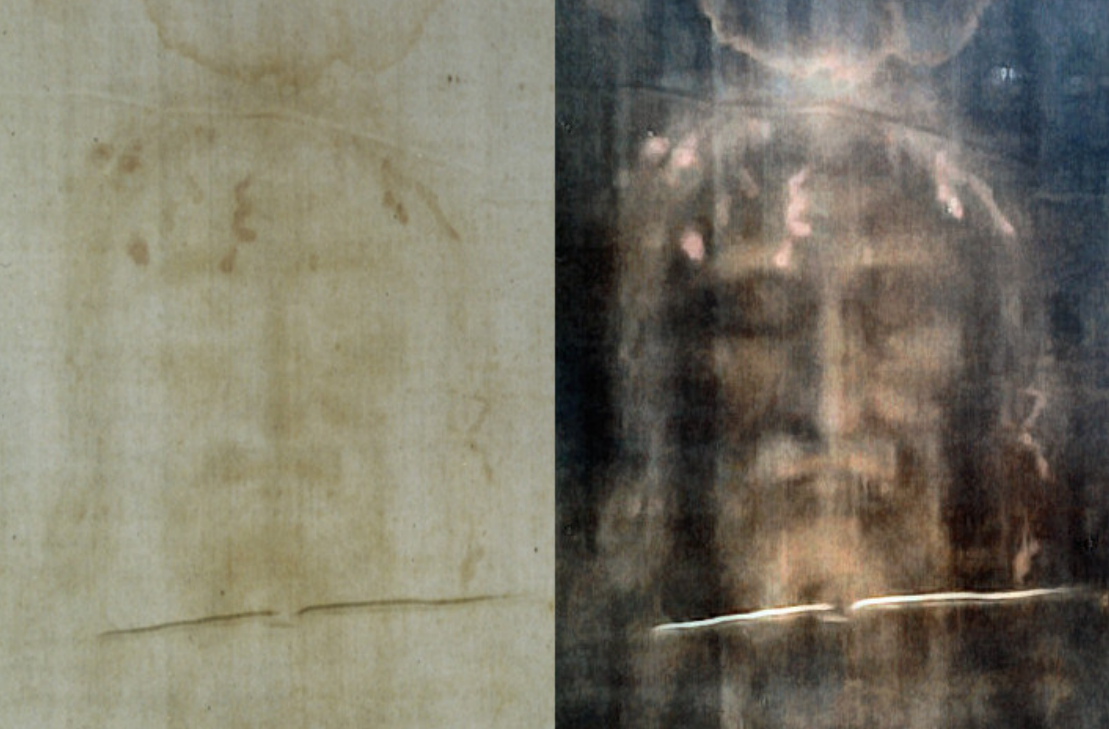
\includegraphics[width=0.7\textwidth]{img/sabanaSanta.png}
\end{figure}
Figura 1: La sábana de Turín: foto moderna de la cara; el positivo a la izquierda y la imagen digitalmente procesada, a la derecha.\\

En 1988, el Vaticano autorizó que el Museo Británico datara la reliquia conocida como la sábana de Turín, posiblemente el sudario del entierro de Jesús de Nazareth. La sábana tiene impresa la imagen de un cuerpo humano que fue venerada como la de Jesús, aunque en la misma iglesia católica ha habido controversias respecto a su autenticidad. Los resultados del Museo Británico mostraron que el contenido de carbono 14 de la sábana estaba entre el $92 \%$ y el $93 \%$ del correspondiente a una tela recién hecha. Con base en esta información y el dato de que la vida media del carbono 14 es de aproximadamente 5730 años:

\begin{enumerate}	
\item Calcule la cantidad de carbono 14 que debería haberse encontrado en la sábana de Turín en 1988, si hubiera sido tejida en tiempos de Jesús.

Para resolver el problema debemos conocer la fórmula para calcular la cantidad del Carbono 14
\[
f(t)=a_1 \cdot e^{-a_2 \cdot t}
\]
donde $a_1$ y $a_2$ son constantes. En este caso, $a_1$ es la cantidad inicial de Carbono 14 (expresada en porcentaje)
\[
f(t)=100 \cdot e^{-a_2 \cdot t}
\]
Para calcular el valor de la constante $a_2$, utilizaremos el dato de la vida media, el cual expresa lo siguiente $f(5730)=\frac{100}{2}$. Por lo que
\[
\frac{100}{2}=100 \cdot e^{-a_2 \cdot 5730}
\]
\[
\frac{1}{2}=e^{-a_2 \cdot 5730}
\]
\[
ln(\frac{1}{2}) = ln ( e^{-a_2 \cdot 5730} )
\]
\[
ln(2^{-1}) = ln ( e^{-a_2 \cdot 5730} )
\]
\[
-ln(2) = -a_2 \cdot 5730
\]
\[
ln(2) = a_2 \cdot 5730
\]
\[
a_2 = \frac{ln(2)}{5730}
\]
Sustituyendo $a_2$ en la fórmula original, nuestra fórmula para calcular la cantidad del Carbono 14 en base al tiempo queda de la siguiente manera
\[
f(t)=100 \cdot e^{-\frac{ln(2)}{5730} \cdot t}
\]
Si $t=1988$
\[
f(1988)=100 \cdot e^{-\frac{ln(2)}{5730} \cdot 1988}
\]
\[
f(1988)=100 \cdot e^{-0.24048}
\]
\[
f(1988)=100 \cdot 0.78624
\]
\[
\therefore f(1988)=78.624\%
\]

\item Explique por qué los arqueólogos del Museo Británico dictaminaron que la tela del sudario debió haberse tejido entre 1299 y 1380.

\item Dé su opinión sobre la siguiente afirmación: “ únicamente un milagro explicaría que la imagen impresa en la sábana de Turín sea la de Jesús de Nazareth”.

\end{enumerate}



\section{La malahora del occiso}
Flores Morán Julieta Melina\\
\\
Según la ley de enfriamiento de Newton, si un cuerpo con temperatura inicial $T (0) = T_0$ se
sumerge en un medio cuya temperatura ambiente $T_a$ permanece constante, donde $T_0 > T_a$, la
temperatura $T(t)$ del cuerpo en el momento $t$ viene dada por la función: \\
(1)\\
\[
T(t)= T_a + (T_0-T_a)e^{-kt},
\]
donde k es una constante positiva.\\ \\
El cadáver de una víctima de asesinato es descubierto a la media noche y, en ese momento,
el médico forense registra que la temperatura del cuerpo es de $31  ^{\circ} C$ y, una hora más tarde, la temperatura del cadáver es de $29  ^{\circ} C $. 
Si se supone que la temperatura del aire circundante permanece constante a $21 ^{\circ}  C$ y que la temperatura "normal" de un ser humano vivo es de $37  ^{\circ} C$, con base en estos datos y la ley de enfriamiento de Newton, calcular la hora en que ocurrió el asesinato. Para ello, siga este procedimiento:
\begin{enumerate}
\item Suponga que $t = 0$ es el momento en que se encuentra el cadáver. Identifique los valores
correspondientes a $T_0$ y $T_a$ de este problema y sustitúyalos en la ecuación (1) para obtener
que, en este caso:
\[
T_0 = Temperatura \;a \;la\; media \;noche= 31  ^{\circ} C
\]
\[
T_a = Temperatura \;del \;ambiente = 21 ^{\circ}  C
\]
Remplazando estos valores se tiene que : 
\[
T(t)= 21 + (31-21)e^{-kt}
\]
(2)
\[
\therefore  T(t)= 21 + 10e^{-kt}
\]  
\item Para determinar el valor de $-k$, tome en cuenta que $T(1) = 29$, sustituya $t = 1$ en la ecuación (2) y despeje $k$ para mostrar que:
\[
 T(1)= 21 + 10e^{-k} = 29
\]  
\[
 10e^{-k} = 29-21
\]  
\[
  e^{-k} = \frac{8}{10}
\]  
\[
 -k = ln\frac{8}{10}
\]  
\[
 \therefore  k = -ln\frac{8}{10} = 0.2231435513
\] 
\item Sustituya el valor de $-K$ en la ecuación (2) para obtener la ecuación de enfriamiento del
cadáver:\\
(3)
\[
T(t)= 21 + 10e^{-0.2231435513t}
\] 
\item Por último, use el dato de que en el momento de la muerte, la víctima tenía una temperatura
corporal de $37  ^{\circ} C$ para concluir que el asesinato ocurrió a las 21 : 54 horas; es decir, dos horas y seis minutos antes de la media noche.
\\
Para conocer el tiempo transcutido dada una temperatura, necesitamos la inversa de esta función, la cúal tendrá como variable independiente la temperatura y variable dependiente el tiempo transcurrido. \\
Despejamos t para conocer la inversa de: 
\[
T= 21 + 10e^{-0.2231t}
\] 
Entonces
\[
\frac{T-21}{10}= e^{-0.2231t}
\] 
\[
ln \frac{T-21}{10}= -0.2231t
\] 
\[
t = -ln \frac{T-21}{10} \times \frac{1}{0.2231}
\]
\[
\therefore T^{-1}(t) = -ln \frac{t-21}{10} \times \frac{1}{0.2231}
\]
$T^{-1}$ es la función inversa , dada una t que es la temperatura de la que se quiere saber el tiempo transcurrido.\\
Para  $37  ^{\circ} C$:
\[
T^{-1}(37) = -ln \frac{37-21}{10} \times \frac{1}{0.2231} = -2.106694
\]
Este resultado indica que los $37  ^{\circ} C$ fue la temperatura de cuerpo 2.106694 horas antes de $T_0$ que se tomó a la media noche.\\
Considerando que:
\[
	0.106694\;h \;(\frac{60 \; min}{1\; hora}) = 6.4016 minutos
\]
\[
2.106694 \; horas \approx 2 \;horas \;y \;6 \;minutos
\]
Por lo tanto, podemos saber que el asesinato fue a las 00:00 horas menos 2 horas y 6 minutos, es decir, 21:54 horas.
\end{enumerate}
\end{document}